\section{Реализация}

\subsubsection*{Анализатор:}
В компании есть работающий анализатор, основанный на абстрактной интерпретации. Поддерживаемые языки - JavaScript, TypeScript. Анализируемый код транспилируется при помощи Babel в промежуточное представление (intermidiate representation). Затем IR с помощью antlr переводится в Control Flow Graph (CFG)

\begin{figure}[H]
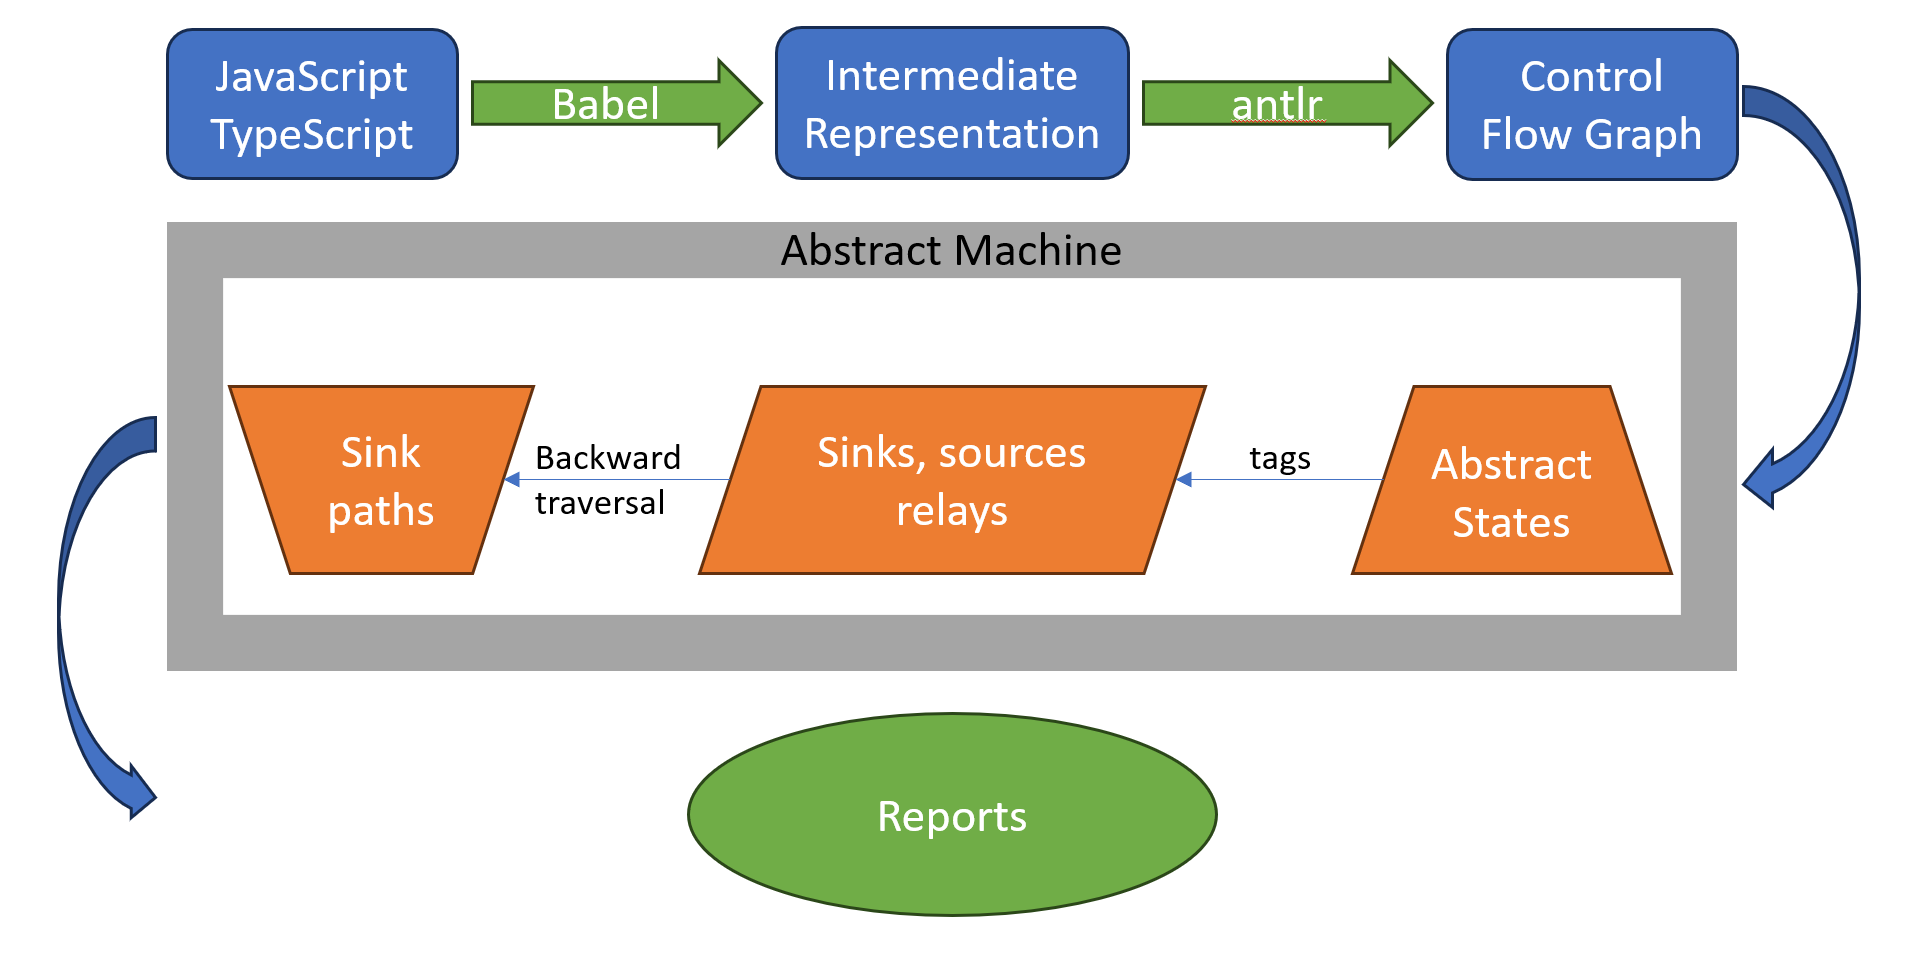
\includegraphics[width=\textwidth]{images/engine.png}\hfill
\end{figure}

Этот граф передается в абстрактную машину, которая обычные переменные переводит в абстрактные, то есть принимающие множество возможных значений. Далее применяется Taint анализ, и в результате для каждой уязвимости выводится весь путь

\newpage
\subsubsection*{Необходимо реализовать:}
Реализован интерфейс для решёток, интервальная решетка для целых чисел и строковая решётка из JSAI, которую необходимо улучшить\\ \\
В новой версии решетки должны присутствовать:
\begin{itemize}
    \item Структура автомата, функции для работы с ним
    \item Общие операции для решеток (join, meet, strictEquals, ...)
    \item Операции на строках (length, concat, substring, ...)
    \item Оператор замыкания (widening)
\end{itemize}
На существующем бенчмарке из 85 реальных проектов:
\begin{itemize}
    \item Суммарное время анализа не должно увеличиться более чем на $20\%$
    \item Потребление памяти не должно увеличиться более чем на $10\%$
\end{itemize}



\newpage
\subsection{Структура}
Сама структура автомата базовая - есть вершины (states) и переходы между ними. Некоторые из стейтов помечены как начальные или как конечные. На переходах стоят строки или символ $\top$, обозначающий любую строку

% \subsubsection*{Операции над множествами строк}
\subsubsection*{union}
Основной операцией является объединение автоматов. С её помощью находим наименьший язык, содержащий оба, порождаемых автоматами

Реализаиця простая: создаем общее начальное состояние, проводим из него переходы с пустой строкой в начальные состояния двух объединяемых автоматов. Затем минимизируем полученный автомат (чуть ниже описана функция minimize)

\subsubsection*{intersect}
Еще одной важной операцией является пересечение автоматов. Она позволяет понять, есть ли в двух алфавитах общие слова. А также находить наибольший общий подъязык

Реализуется она при помощи операций дополнения и объединения, то есть по формуле \[A \cap B = S / ((S / A) \cup (S / B))\]

Дополнение строится таким образом - выписываем все возможные переходы в обоих автоматах, а затем для каждого переходы между двумя вершинами заменяются на дополнение к этим переходам

\subsubsection*{subset}
Проверка на то, что один язык полностью содержит другой. Реализуется с помощью дополнения и пересечения по формуле
\[A \subset B <=> (S / B) \cap A = \emptyset\]

\subsubsection*{minimize}
Убирает лишние вершины и переходы. Например может произойти так, что из одной вершины ведут 2 перехода с одинаковой строкой. Тогда можно упростить автомат так, чтобы склеились 2 вершины в одну. Также избавляемся от переходов по пустой строке

Алгоритм минимизации такой - сначала проверяем, является ли автомат детерменированным, то есть что нет двух исходящих переходов из одной вершины с одинаковыми символами на них. А также что нет пустых переходов. Если есть, то склеиваем эти 2 вершины. Это операция детерменирования

Затем, чтобы избавиться от двух одинаковых входящих переходов, мы делаем reverse, то есть перенаправляем все ребра и помечаем конечные вершины начальными и наоборот. Теперь вызываем еще раз determinize. Повторив еще раз reverse + determinize, получим начальный автомат, но без лишних переходов и вершин

Последним шагом удаляем те вершины, из которых нельзя попасть в финальные. Таким образом получим упрощенную версию того же самого автомата

TODO ПРИМЕР С КАРТИНКАМИ

\subsubsection*{explode}
Для реализации сложных операций на строках, такие как Replace и Substr, в которых нужно искать подстроки в автоматах, есть операция, которая переводит автомат к конечному автомату с переходами по буквам. Она просто заменяет каждое ребро на путь, где на каждом переходе лишь один символ вместо целого слова. Также есть обратная операция, которая схлопывает вершины с одним входящим и одним выходящим ребром в один переход

\subsubsection*{getLanguage}
Собираем все слова, порождаемые автоматом, с помощью прохода DFS. Если в графе есть цикл, то возможных слов бесконечно, и этот случай нужно отдельно разобрать. Эта операция полезна для оптимизаций в некоторых случаях (далее будет пример)

\newpage
\subsection{Операции для решеток}
Операции join и meet аналогичны union и intersect для автоматов. Остается только разобрать случаи, когда один из аргументов $\top$ или $\bot$. 

\subsubsection*{equals}
Проверяем, что 2 автомата порождают одинаковые языки. В общем случае можем проверить то, что один язык включается в другой (subset) и наоборот. Однако операция пересечения слишком громоздкая (нужно сделать 3 раза дополнение), поэтому для конечных языков проще выписать 2 порождаемых языка и проверить их на соответствие. Язык является конечным, если в нем нет $\top$ переходов и циклов

\subsubsection*{strictEquals}
В отличие от equals, strictEquals проверяет то, что есть хоть одно общее слово. Опять это можно сделать при помощи пересечения, то есть что пересечение не пусто. Но для конечных лучше сравнивать языки





\newpage
\subsection{Операции на строках}
\subsubsection*{Length}
Возвращает интервал $[c_1, c_2]$, такой что $c_1 \leq |s| \leq c_2$. При этом если $s$ содержит в себе цикл, или же содержит в себе переход, на котором стоит $\top$, то есть любая строка, то максимальная длина будет сколь угодно большой. Минимальная при этом заменяет все топы на пустые строки
$$
\text{length}(s) \triangleq 
\begin{cases}
[\lvert \text{minPath}(A) \rvert, +\infty] & \text{if } \text{cyclic}(A) \lor \text{readsTop}(A) \\
[\lvert \text{minPath}(A) \rvert, \lvert \text{maxPath}(A) \rvert] & \text{otherwise}
\end{cases}
$$

Для подсчета длины запускаем DFS из начальных стейтов. При вхождении в терминальный, считаем длину пути (заменяя $\top$ на $0$ или $+\infty$ соответственно) и пересчитываем максимальную и минимальную длину

Если автомат содержит в себе цикл, то с помощью DFS мы его найдем и максимальная длина пути будет бесконечной, так как можно по этому циклу крутиться сколь угодно много раз

\subsubsection*{Concat}
При конкатенации достаточно добавить для первого автомата одну дополнительную конечную вершину, в которую будут вести переходы с пустой строкой из конечных вершин первого, а затем из нее ведут переходы в начальные вершины второго автомата. Далее стоит минимизировать полученный автомат, чтобы избавиться от пустых ребер

\newpage
\subsubsection*{Contains}
Абстрактная семантика contains должна возвращать значение true, если любая строка из A' содержится в любой строке из A, значение false, если какая-то строка из A' не содержится в какой-то строке из A и \{true, false\} ($\top$) в остальных случаях

$$
\text{contains}(s, s') \triangleq 
\begin{cases}
\text{false} & \text{if } A' \sqcap \text{FA}(A) = \text{Min}(\emptyset) \\
\text{true} & \text{if } \neg \text{cyclic}(A) \land \text{singlePath}(A') \\
& \land \forall \pi \in \text{paths}(A). \sigma_{sp} \curvearrowright_s \sigma_{\pi} \\
\{ \text{true}, \text{false} \} & \text{otherwise}
\end{cases}
$$

Для начала определим, в каком случае нужно возвращать false. Для этого определим фактор-автоматон FA(A), который принимает все подстроки A. Для этого нужно просто пометить все стейты конечными. Затем пересечь FA(A) и A', чтобы проверить, что никакая подстрока любой строки из A не является строкой из A'

Теперь, в каком случае true. Если A' содержит 2 слова, ни одно из которых не является префиксом другого, то они оба не могут быть одновременно префиксами какого-либо слова из A. Значит все слова в A' должны быть по цепочке включены друг в друга. Или же автомат для них выглядит как путь, некоторые вершины на котором конечные. И в этом случае достаточно проверить, что самое длинное слово входит во все слова из A, тогда и его префиксы будут

Во всех остальных случаях точного ответа нет, поэтому возвращаем $\top$

\newpage
\subsubsection*{Substr, Replace, IndexOf}
Все 3 функции похожи друг на друга тем, что нужно искать в автомате подстроки по определенным условиям. И так как на переходах стоят не символы, а строки, то подстрока может заканчиваться или начианться где-то в середине этого перехода. Чтобы избежать такого, первым шагом вызывается explode, чтобы начало и конец всегда были в вершинах

Следующий шаг также общий, а именно обход графа в глубину и запоминание тех путей из начальных вершин в конечные, которые содержат в себе интересующую подстроку (это может быть вхождение подстроки в этот путь в случае Replace или indexOf, или же просто возможность взять подстроку нужной длины для Substr)

А вот далее нужно полученные пути склеить в один автомат. Для этого добавляем одну общую начальную и конечную вершину, к ним присоединяем начала и концы путей, и затем минимизируем. Чтобы привести полученный автомат к сокращенному виду, а именно со словами на ребрах, делаем операцию обратную explode, то есть схлопываем вершины, у которых одно входящее и одно выходящее ребро. Получаем искомый автомат

Есть сложность в том, что автомат может содержать в себе цикл. В этом случае обход в глубину не сможет вернуть все пути, так как их бесконечно много. И обрабатывать цикл на то, можно ли с его помощью накрутить подстроку, подходящую под условия, не получится из-за предпериода или еще одного цикла (какой сколько раз крутить непонятно). В случае с Substr можно обрезать пути по длине, но для indexOf и Replace так не получится. Поэтому в данном случае приходится возвращать $\top$

Вот краткое описание indexOf, более подробное описание всех операций можно найти в статье~\cite{tarsis2021}

$$
\text{indexOf}(s, s') \triangleq 
\begin{cases}
[-1, +\infty] & \text{if } \text{cyclic}(A) \lor \text{cyclic}(A') \lor \text{readsTop}(A') \\
[-1, -1] & \text{if } \forall \sigma' \in \mathcal{L}(A') \text{ } \nexists \sigma \in \mathcal{L}(A). \sigma' \curvearrowright_s \sigma \\
\underset{\sigma \in \mathcal{L}(A')}{\bigsqcup} \text{IO}(A, \sigma) & \text{otherwise}
\end{cases}
$$

\subsection{Остальные операции}
В статье TARSIS описан алгоритм только для 6 операций, тогда как на деле их гораздо больше. Часть из них похожа на описанные сверху, какие-то понятно как реализовывать. Но есть и более сложные. Разберем некоторые из них

\subsubsection*{startsWith, endWith}
Идем из начальных (или конечных в случае endWith) вершин, ища те переходы, чтобы путь совпадал с паттерном. Если не находим такого пути, значит точно false. Если оказывается, что путь нужной длины только один, значит true. Иначе $\top$

\subsubsection*{charAt, slice, includes}
Эти функции похожи на substr, аналогично шагаем по путям на нужную длину. В случае с charAt проверяем, что все символы на нужном месте одинаковые и равны нужному (true), либо что ни один не равен (false), в остальных случаях $\top$. Для slice вырезаем нужную часть автомата аналогично substr

Includes аналогична indexOf, только нужно возвращать не индекс, а true/false

\subsubsection*{trim, toUpperCase, pad, match}
Первые 2 функции легко реализуются, нужно просто проделать операцию для каждого перехода. А вот pad и match сходу непонятно, как реализовывать для автоматов. Одной из проблем является например $\top$ ребро, которое не дает определить длину слова и непонятно, сколько символов вставлять в начало. И один из несложных вариантов реализации это выписать весь язык, порождаемый автоматом, для каждого слова по отдельности проделать операцию и склеить в один автомат. Такой подход все также плохо будет работать с циклами, то есть для цикличных автоматов возвращаем $\top$

\subsubsection*{toNum, toBool}
toBool проверяет то, есть ли в языке пустая строка или "0". Если нет, то true. Если язык состоит только из пустой строки или "0", то false, иначе $\top$

toNum должен вернуть в результате интервальную решетку для чисел, то есть ограничение сверху и снизу на значение. И заодно проверить, что все строки состоят из корректных символов, то есть цифр, не более одной точки или запятой и возможно минус в начале. Также перебираем всевозможные пути, проверяем на корректность. Запоминаем минимальное и максимальное значение

В случае с toNum $\top$ переход является недопустимым, так как это любой символ, в том числе буква. Но вот с циклами можно работать. Сначала нужно понять, находится ли эта часть строки после точки, или нет. Если нет, значит число может неограниченно расти и стремиться к $\pm \infty$. А для поиска минимального цикл нужно прокрутить только 1 раз. Если бесконечная часть появляется после точки, значит достаточно прибавить $0.1$ к числу и обрезать хвост, ибо в любом случае получим ограничение сверху

\newpage
\subsection{Оператор расширения}
Важным методом является оператор расширения (widening). Именно благодаря ему удается завершать циклы за конечное время, создавая аппроксимацию. Рассмотрим пример того, как это реализованно

\begin{lstlisting}[caption={Пример применения widening}]
function f(v) {
    res = "";
    while(?) res = res + "id = " + v;
    return res;
}
\end{lstlisting}

Автомат, задающий значения res в начале второй итерации цикла while, выглядит так:
\begin{figure}[h]
    \centering
    \begin{tikzpicture}[->, >=stealth', shorten >=1pt, auto, node distance=3cm, semithick]
        \node[state, initial, accepting] (q0) {$q_0$};
        \node[state, right of=q0] (q1) {$q_1$};
        \node[state, right of=q1, accepting] (q2) {$q_2$};
        
        \path (q0) edge node[above] {id = } (q1)
                (q1) edge node[above] {$\top$} (q2);
    \end{tikzpicture}
\end{figure}

В конце второй итерации вот так:
\begin{figure}[h]
    \centering
    \begin{tikzpicture}[->, >=stealth', shorten >=1pt, auto, node distance=3cm, semithick]
        \node[state, initial] (q0) {$q_0$};
        \node[state, right of=q0] (q1) {$q_1$};
        \node[state, right of=q1, accepting] (q2) {$q_2$};
        \node[state, right of=q2] (q3) {$q_3$};
        \node[state, right of=q3, accepting] (q4) {$q_4$};
        
        \path (q0) edge node[above] {id = } (q1)
                (q1) edge node[above] {$\top$} (q2)
                (q2) edge node[above] {id = } (q3)
                (q3) edge node[above] {$\top$} (q4);
    \end{tikzpicture}
\end{figure}

Далее, для этих двух автоматов приминяем саму операцию расширения. Алгоритм такой:
\begin{itemize}
    \item Делаем union для этих автоматов:
    \begin{figure}[h]
        \centering
        \begin{tikzpicture}[->, >=stealth', shorten >=1pt, auto, node distance=3cm, semithick]
            \node[state, initial, accepting] (q0) {$q_0$};
            \node[state, right of=q0] (q1) {$q_1$};
            \node[state, right of=q1, accepting] (q2) {$q_2$};
            \node[state, right of=q2] (q3) {$q_3$};
            \node[state, right of=q3, accepting] (q4) {$q_4$};
            
            \path (q0) edge node[above] {id = } (q1)
                    (q1) edge node[above] {$\top$} (q2)
                    (q2) edge node[above] {id = } (q3)
                    (q3) edge node[above] {$\top$} (q4);
        \end{tikzpicture}
    \end{figure}

    \newpage
    \item Стейты, у которых исходящие пути длины 2 совпадают, объединяем. В данном случае $q_0$ и $q_2$ оба принимают $id = \top$, и потому склеиваются в одну вершину:
    \begin{figure}[h]
        \centering
        \begin{tikzpicture}[->, >=stealth', shorten >=1pt, auto, node distance=3cm, semithick]
            \node[state, initial, accepting] (q0) {$q_0, q_2$};
            \node[state, right of=q0] (q1) {$q_1$};
            \node[state, below of=q1] (q3) {$q_3$};
            \node[state, right of=q3, accepting] (q4) {$q_4$};
            
            \path (q0) edge node[above] {id = } (q1)
                    (q0) edge node[right] {id = } (q3)
                    (q1) edge[bend left] node[above] {$\top$} (q0)
                    (q3) edge node[above] {$\top$} (q4);
        \end{tikzpicture}
    \end{figure}

    В общем случае длину пути для склейки вершин можно регулировать, чем она больше, тем точнее результат, однако и размер автомата больше
    \item Минимизируем полученный автомат:
    \begin{figure}[h]
        \centering
        \begin{tikzpicture}[->, >=stealth', shorten >=1pt, auto, node distance=3cm, semithick]
            \node[state, initial, accepting] (q0) {$q_0$};
            \node[state, right of=q0] (q1) {$q_1$};
            
            \path (q0) edge node[above] {id = } (q1)
                    (q1) edge[bend left] node[above] {$\top$} (q0);
        \end{tikzpicture}
    \end{figure}
\end{itemize}

Теперь заметим, что полученный автомат является неподвижной точкой. Для этого попробуем проделать ещё одну итерацию цикла. После объединения автоматов в начале и конце цикла получаем такой:

\begin{figure}[h]
    \centering
    \begin{tikzpicture}[->, >=stealth', shorten >=1pt, auto, node distance=3cm, semithick]
        \node[state, initial, accepting] (q0) {$q_0$};
        \node[state, right of=q0] (q1) {$q_1$};
        \node[state, right of=q1, accepting] (q2) {$q_2$};
        
        \path (q0) edge node[above] {id = } (q1)
                (q1) edge[bend left] node[above] {$\top$} (q0)
                (q1) edge node[above] {$\top$} (q2);
    \end{tikzpicture}
\end{figure}

Склеивать вершины не придется, однако при минимизации $q_0$ и $q_2$ станут одной, то есть получим начальный автомат, что означает отсутствие изменений и значит можно остановиться 

Доказано~\cite{widening}, что такой алгоритм расширения соответствует условиям овер-аппроксимации


\newpage
\subsection{Тестирование}
Были написаны тесты на новую финкциональность, разберем несколько примеров

\begin{lstlisting}[caption={Пример CWE тестов}]
function tossCoin(): string {
    if (Math.Random() > 0.5) {
        return "eagle"
    } else {
        return "tails"
    }
}

if (tossCoin() == "edge") {
    /* POTENTIAL FLAW GOOD: */
    console.log(document.getElementById('source').value)
}
\end{lstlisting}
    
В данном примере в консоль выводятся помеченные данные (то есть те, которые влекут за собой уязвимость), если выполняется условие. Для определения абстрактного значения tossCoin(), происходит join двух веток исполнения. В старой строковой решетке результатом был класс обычных строк (NotNumNorSpl). Однако, edge также может принадлежать этому классу, из-за чего сравнение на эквивалентность строк должно возвращать $\top$, что есть возможно true и false. И тогда ветка исполнения, в которой в консоль выводятся опасные данные, также возможна. И значит анализатор указывал на то, что в этой строчке возможна уязвимость, тогда как на деле этого не происходит

С новой решеткой мы точно можем сказать, что ни одно возвращаемое знаение функции tossCoin не равно edge, а следовательно мертвый код игнорируется. Потому можем поставить метку POTENTIAL FLAW GOOD, означающую отсутствие уязвимости

\newpage
\begin{lstlisting}[caption={Пример IR тестов}]
function tossCoin(): string {
    if (Math.Random() > 0.5) {
        return "eagle"
    } else {
        return "tails"
    }
}

let x = tossCoin()
console.log(x.indexOf("a")) // [number: [1, 1]]
console.log(x.indexOf("e")) // [number: [-1, 4]]
console.log(x.indexOf("r")) // [number: [-1, -1]]
\end{lstlisting}

Другой пример тестов это IR (intermidiate representation) тесты. Они проверяют то, какие абстрактные значения принимают переменные. По аналогичным причинам старая решетка не могла как либо оценить значение indexOf. Новая же позволяет это сделать. Благодаря этому, не только строковые значения стали более точными, но и некоторые числовые


\begin{lstlisting}[mathescape=true, caption={Еще пример IR тестов}]
var x = "a" + document.getElementById('source').value + "c"
console.log(x)                 // [string: a$\top$c tags=[XSS,WEB]]
console.log(x.length)          // [number: [2, +Inf]]
console.log(x.startsWith("a")) // [boolean: true]
console.log(x.substr(0, 1))    // [string: a tags=[XSS,WEB]]
\end{lstlisting}

В данном примере видно, что даже если в операциях участвует $\top$, все еще можно знать что-то о строке, как напимер минимальную длину или то, что startsWith('a') это всегда true

Также можно увидеть tags=[XSS,WEB]. Это как раз и есть метка, которая указывает на уязвимые данные. И при некоторых операциях она сохраняется, как например конкатенация. Одним из уточнений в будущем может стать то, что эта метка будет принадлежать конкретному переходу, а не всему абстрактному значению. То есть например если сейчас сделать x.substr(0, 1), то результат будет 'a', то есть вообще не содержать опасных символов. Однако метка будет передана


\newpage
\subsection{Результаты}
Для подсчета итоговой статистики были произведены запуски анализатора с использованием старой и новой решеток на внутренних тестовых проектах, а также на Open Surce JavaScript проектах для парсинга текстов и сериализации, то есть те, где большое использование строковых переменных в коде 

Разберем результаты на примере 3-х различных по размеру проектов:

\subsubsection*{SceneBoard}
Самый большой проект в пуле тестовых. Размер 250к строк. Время анализа составило 506к ms (8 минут 26 секунд) на старой решетке и 526к ms (8:46) на новой, то есть прирост 4\%. Потребление памяти было 17935 МБ на старой и 16706 МБ на новой, то есть уменьшилось на 7\%. Снижение обусловлено тем, что благодаря повышению точности было проигнорировано больше строчек кода, так как он мертвый, то есть никогда не запускается в реальности. Замеры точности можно увидеть в табличке снизу

TODO табличка

\subsubsection*{Notepad}

\subsubsection*{AppGalery}

\subsubsection*{Open Source}
